\chapter{Kravspecifikation (SK)}

Der er blevet udarbejdet en kravspecifikation ud fra følgende use cases se figur \ref{lab:usecasediagram}, her er der beskrevet hvilke use cases brugeren, DE2 boardet, eksterneenheder, barn og SMS-modtager har kontakt med. 

\begin{figure}[!htbp] \centering
\section{Usecases}
\vspace*{\fill}
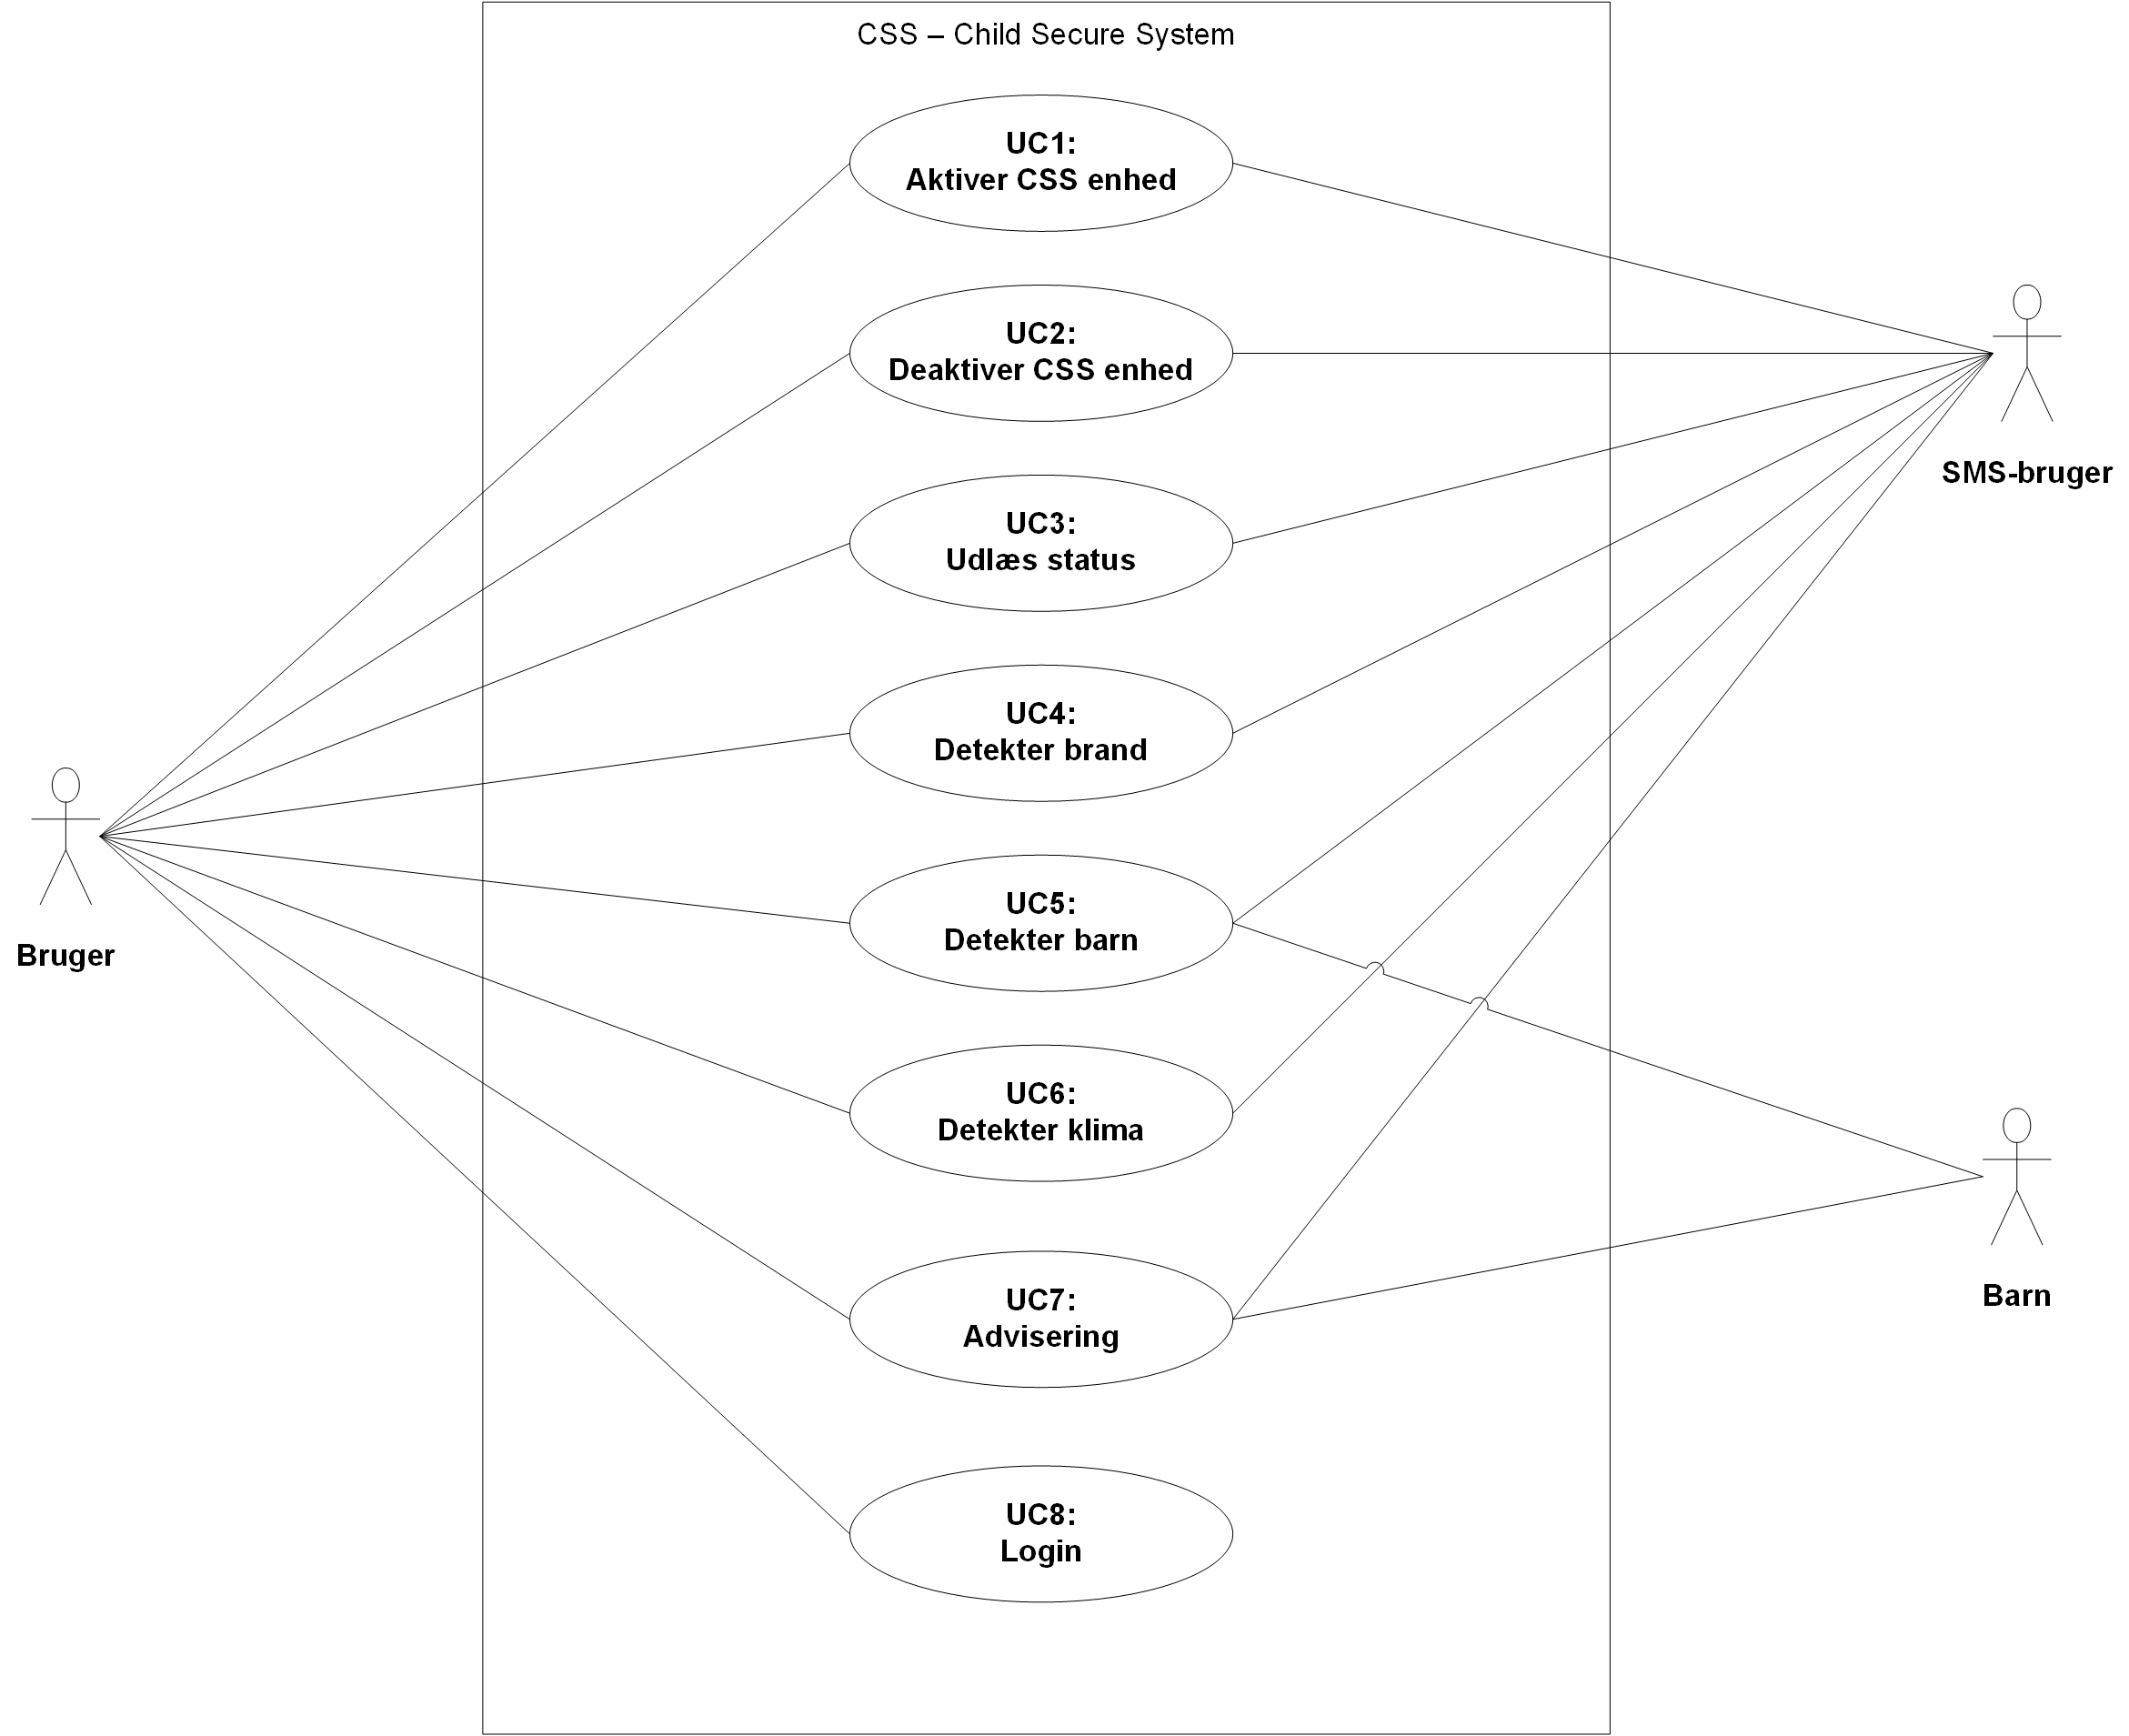
\includegraphics[width=\textwidth]{billeder/diagrammer/Usecase_Diagram}
\caption{Usecase diagram}
\label{lab:usecasediagram}
\vspace*{\fill}
\end{figure}

For yderligere beskrivelse af hver enkelt use case og større forståelse henvises til projektdokumentation\footnote{Projektdokumentation s 9-18}
\newpage

Herunder ses en beskrivelse af hver enkelt aktør i systemet.

\begin{table}[!htbp] \centering
\subsection{Bruger}
\begin{tabular}{|p{4cm}|p{8cm}|}
	\hline
		\textbf{Type Beskrivelse} &
			Bruger aktøren er ejeren af systemet eller den voksne med adgang til Computeren. 
			Vil typisk være forældre, barnepige osv. (Primær) \\\hline
	\end{tabular}
\end{table}

\begin{table}[!htbp] \centering
\subsection{Eksterne enheder}
\begin{tabular}{|p{4cm}|p{8cm}|}
	\hline
		\textbf{Type Beskrivelse} &
			Eksterne enheder, omfatter hvad man ønsker at aflåse eller slukke for. 
			Vil typisk være skabe, komfur, el-kedel osv. (Sekundær) \\\hline
	\end{tabular}
\end{table}

\begin{table}[!htbp] \centering
\subsection{Barn}
\begin{tabular}{|p{4cm}|p{8cm}|}
	\hline
		\textbf{Type Beskrivelse} &
			Barnet eller børnene i huset, som systemet skal beskytte.	(Sekundær) \\\hline
	\end{tabular}
\end{table}

\begin{table}[!htbp] \centering
\subsection{SMS modtager}
\begin{tabular}{|p{4cm}|p{8cm}|}
	\hline
		\textbf{Type Beskrivelse} &
			Typisk forældrene eller barnepigen. Den person der skal have besked om gråd eller anden støj fra børneværelset. (Sekundær) \\\hline
	\end{tabular}
\end{table}

\begin{table}[!htbp] \centering
\subsection{DE2 Board}
\begin{tabular}{|p{4cm}|p{8cm}|}
	\hline
		\textbf{Type Beskrivelse} &
			DE2 Board programmeret som kodelås i DSD øvelse 7 (Sekundær) \\\hline
	\end{tabular}
\end{table}


\subsection*{Ikke-funktionelle krav}
Herunder ses en beskrivelse af ikke-funktionelle krav.

\begin{enumerate}
	\subsection*{Brugbarhed (Usability)}
	\item UI skal kunne bruges efter gennemlæst manual.


	\subsection*{Pålidelighed (Reliability)}

	\item Levetid: 5 år uden hardware nedbrud
	\item Software oppetid: Minimum 1 måned før genstart


	\subsection*{Ydeevne (Performance)}
	\item System respons må maksimalt være 2,5 sekunder
	\item Startuptid fra power-off til funktionel tilstand maksimalt 2 minutter
	\item Systemkapaciteten er på maksimalt 15 CSS udtag
	\item Ved lyddetektion må der maksimalt gå 1 minut før SMS-besked er afsendt

	\subsection*{Vedligeholdelse (Supportability)}
	\item X10 udtag kan udskiftes separat ved simpel omkodning ved hjælp af adresseswitchen 
	\item Systemet er plug’n’play i en almindelig husholdning
	\item X10 udtag kan tilføjes og installeres løbende

\subsection*{Generelle krav}
	\item Systemet skal virke på det eksisterende 230 Vac netværk i almindelige husstande
	\item Kommunikationen mellem X10 udtag og hovedenheden skal ske på X10 protokollen
	\item Systemet skal kunne afsende SMS-beskeder
	\item Systemet skal automatisk logge ud efter 1min uden aktivitet

	\subsection*{CSS enheder}
	\item Udtag skal kunne være i en 1,5 moduls Fuga stikdåse
	\item Udtag skal have en LED indikator som viser at den er aktiv
	\item Hovedenheden skal kunne virke på 230 Vac/13 A tilslutning

	\subsection*{Eksterne enheder}
	\item Lyddetektoren skal registrere lyde på over 68 dB
	\item Der må maksimalt afsendes 1 SMS-besked pr. minut ved gentagende reaktion fra lyddetektoren
	\item Låse enheder må maksimalt være 8x5x3 cm
	\item Låse enhederne skal kunne holde 5 kilogram

\end{enumerate}

